\documentclass[a4paper,12pt]{article}
\usepackage[T1,T2A]{fontenc}
\usepackage[utf8]{inputenc}
\usepackage[english,ukrainian]{babel}


\usepackage{ upgreek }
\usepackage{amsmath}

\usepackage{graphicx}
\graphicspath{{./pictures/}}


\usepackage[unicode=true,colorlinks=true,urlcolor=blue,citecolor=green,linkcolor=blue]{hyperref}
\usepackage[ukrainian,nameinlink]{cleveref}
\usepackage{geometry} % Меняем поля страницы
\geometry{left=2cm}% левое поле
\geometry{right=1.5cm}% правое поле
\geometry{top=1cm}% верхнее поле
\geometry{bottom=2cm}% нижнее поле



\begin{document}
	
	\begin{titlepage}
		\vspace*{6cm}
		\begin{center}
			
			\large
			\textbf{Звіт}\\
			\textbf{до лабораторної роботи №2:}\\
			\textbf{<<Побудова діаметра множини>>}
			
		\end{center}
		
		\vspace{8cm}
		\begin{flushright}
			студента 1-го курсу магістратури\\
			факультету комп'ютерних наук та кібернетики\\
			Кравця Олексія
		\end{flushright}
		
	\end{titlepage}

\newpage
\tableofcontents
\newpage
%document here
\section{Постановка задачі}

Маємо множину точок на площині. Необхідно побудувати діаметр цієї множини трьома методами

\begin{itemize}
	\item Алгоритм 1. Жадібний алгоритм. Перебір усіх пар точок.
	\item Алгоритм 2. Побудова опуклої оболонки та алгоритм \cite[\textit{Rotating calipers}]{Rotating calipers}.
	\item Алгоритм 3. Ідея \cite{Cells} алгоритму у побудові клітин, що обмежують кількість точок для перебору.
\end{itemize}

Порівняти швидкість роботи методів.

\section{Алгоритм 2}

Проілюструємо роботу Алгоритму 2.

\begin{figure}[h]
	\center{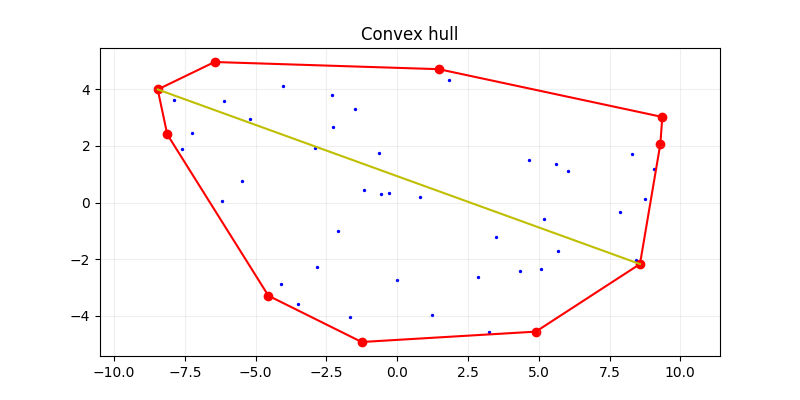
\includegraphics[scale=0.8]{Figure_1.png}}
	\caption{Робота алгоритму 2}
	\label{fig:f1}
\end{figure}

\begin{itemize}
	\item Червоні відрізки та точки -- це відрізки та вершини опуклої оболонки множини.
	\item Сині точки -- точки з множини, що не є вершинами опуклої оболонки.
	\item  Жовтий відрізок -- діаметр множини.
\end{itemize}

\section{Алгоритм 3}

Алгоритм розподіляє множину точок на клітини і викидає клітини, що точно не містять точок, що є вершинами діаметру множини. Такими клітинами є ті, що оточені іншими клітинами з усіх боків. Після цього алгоритм перебирає усі пари точок, що залишилися, для пошуку діаметра. 

Продемонструємо послідовну роботу алгоритму.  
\newpage
\begin{figure}[h]
	\center{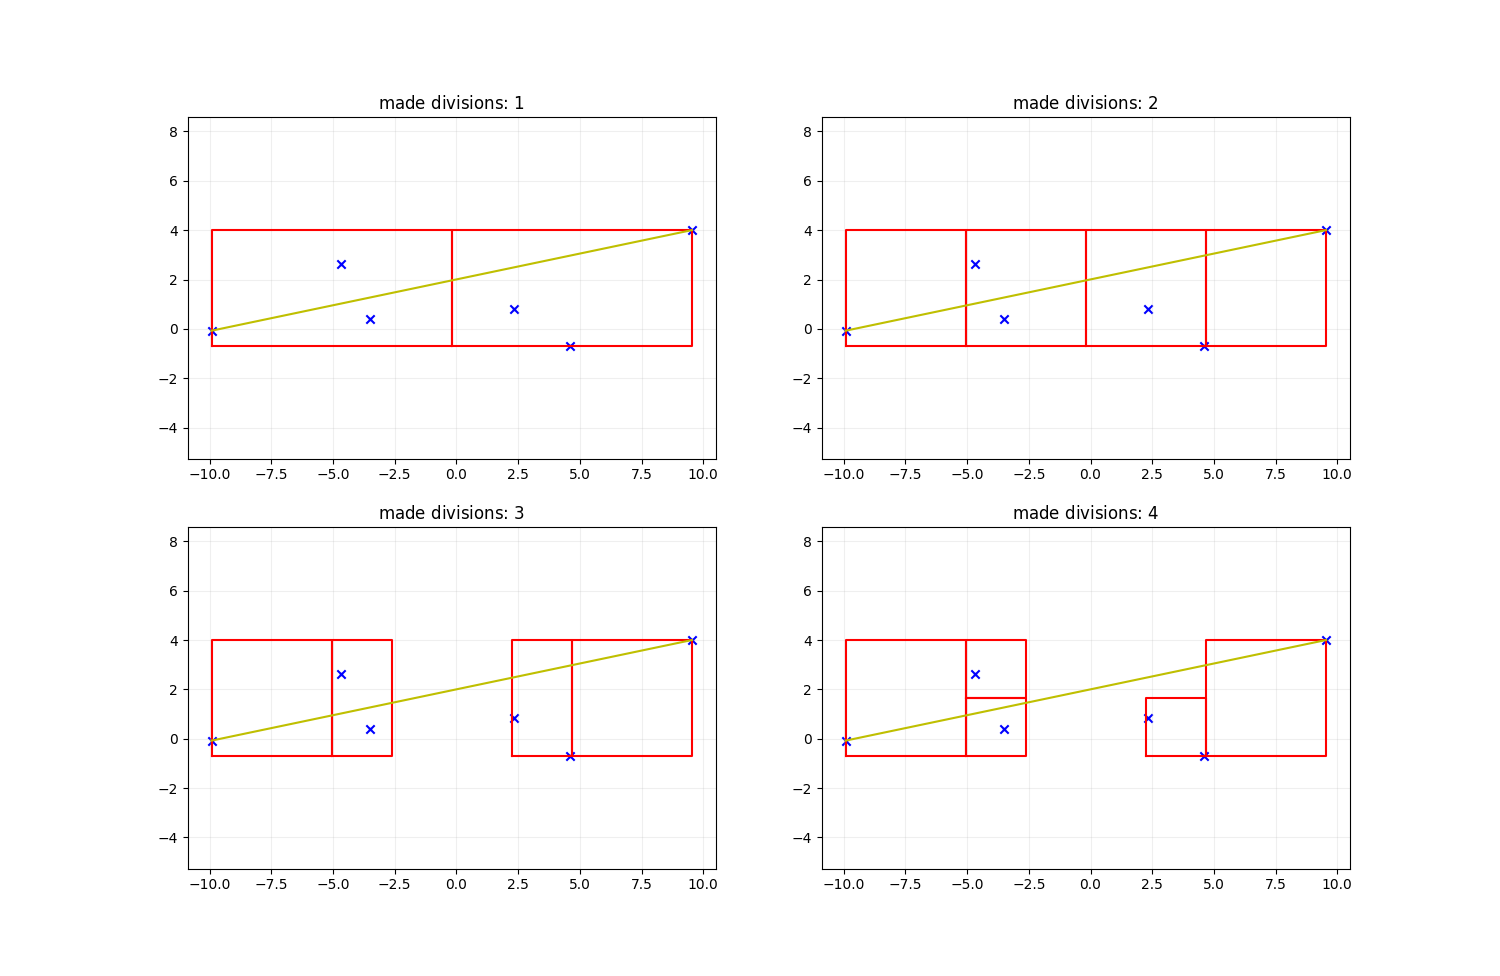
\includegraphics[scale=0.5]{Figure_3.png}}
	\caption{Послідовна робота алгоритму 3}
	\label{fig:f2}
\end{figure}


Ми розділяємо прямокутник, що містить точки на два менші прямокутники, потім ділимо їх аналогічним чином. На кожному кроці ми ділимо усі клітини навпіл та викидаємо з розгляду ті, що точно не містять вершини діаметру множини.

Тепер можна розглянути, як виглядає алгоритм, якщо зробили $10$ розподілів на клітини.

\begin{figure}[h!]
	\center{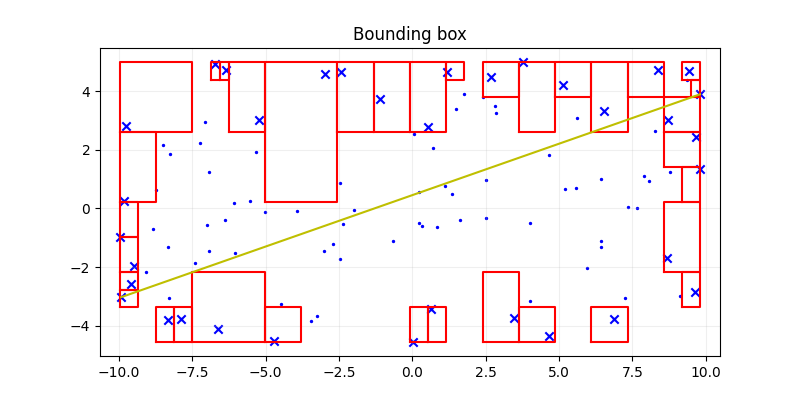
\includegraphics[scale=0.8]{Figure_2.png}}
	\caption{Робота алгоритму 3}
	\label{fig:f3}
\end{figure}

\newpage

На рисунках ми бачимо
\begin{itemize}
	\item Сині точки -- точки множини, що точно не є вершиною діаметра. Їх не будуть розглядати при переборі усіх пар точок.
	\item Сині хрести -- це точки серед яких буде проведений пошук діаметра з використанням жадібного алгоритму.
	\item Червоні прямокутники -- це клітини, що містять необхідні нам точки.
	\item Жовтий відрізок -- діаметр множини.
\end{itemize}


\section{Результати}

$N$ -- кількість точок у множині.Значення в таблиці вказані у секундах. Алгоритм 3 виконував $10$ ділень.

\begin{tabular}{| c | c | c | c | c | c |}
	\hline
	$N$ & 10 & 100 & 500 & 1000 & 5000 \\ 
	\hline
	Алгоритм 1 & 0.0023 & 0.0806 & 2.0422 & 7.9989 & 199.628 \\
	Алгоритм 2 & 0.0016 & 0.011 & 0.0416 & 0.0628 & 0.3105 \\
	Алгоритм 3 & 0.0014 & 0.0107 & 0.0344 & 0.0556 & 2.0986 \\
	\hline
\end{tabular}



\section{Висновки}

За результатами видно, що найбільш ефективним виявився алгоритм 2. Також гарні результати показав алгоритм 3, його можна пришвидшити змінюючи кількість розподілів на клітини. 


\addcontentsline{toc}{section}{Література}
\begin{thebibliography}{}
	\bibitem{Rotating calipers} Shamos, Michael (1978). "Computational Geometry". Yale University. pp. 76–81.
	\bibitem{Cells} Sariel Har-Peled. A Practical Approach for Computing the Diameter of a
	Point Set. March 26, 2001
	\bibitem{} \href{https://en.wikipedia.org/wiki/Rotating_calipers}{https://en.wikipedia.org/wiki/Rotating\_calipers}
\end{thebibliography}

\end{document}
